% Copyright 2021 Joel Feldman, Andrew Rechnitzer and Elyse Yeager, except where noted.
% This work is licensed under a Creative Commons Attribution-NonCommercial-ShareAlike 4.0 International License.
% https://creativecommons.org/licenses/by-nc-sa/4.0/

\documentclass[10pt]{beamer}

 %%%%%%%%%%%%%%%%%%%%%%%%%
 %%%%%%%%%%%%%%%%%%%%%%%%%
 %%%%%%%%%%%%%%%%%%%%%%%%
\usepackage{header101}
\settoggle{spoiler}{true}

\begin{document}

%----------------------------------------------------------------------------------------

%----------------------------------------------------------------------------------------
\begin{frame}{CLP-2 Lecture Slides}
The slides in this folder are written to correspond to \href{https://secure.math.ubc.ca/~CLP/CLP2/}{CLP-2 by Feldman, Rechnitzer, and Yeager}. The slides and their source files can be found online at \url{https://github.com/ecyeager/CLP2Slides}.
\vfill

CLP-2 lecture slides are Copyright 2024 Joel Feldman, Andrew Rechnitzer and Elyse Yeager, except where noted.
They are licensed under a Creative Commons Attribution-NonCommercial-ShareAlike 4.0 International License.
\begin{center}

\includegraphics[height=7mm]{clipart/CC}
\end{center}
\url{https://creativecommons.org/licenses/by-nc-sa/4.0/}
 \end{frame}
%----------------------------------------------------------------------------------------

%----------------------------------------------------------------------------------------
\section{Files}
\frame{\tableofcontents[currentsection]}
%----------------------------------------------------------------------------------------
%----------------------------------------------------------------------------------------
\begin{frame}{Versions} 
Most slides have three versions: \textit{lecture}, \textit{handout}, and \textit{full}.
\begin{description}
\item[lecture] These slides are intended for display and annotation by the instructor during lecture. They include animations, pauses, and space to write solutions to questions. Solutions themselves are generally omitted. 
\item[handout] The handout mode is used to generate slides that students can access before lecture and use to take notes. Most animations and pauses are suppressed. Solutions to questions are also suppressed, so students can work in class without spoilers.
\item[full] These slides are similar to lecture slides, but in addition to including space to write your own solution, they also contain typed solutions. They may be posted to students after class; they may be used by lecturers preparing class; and they may be used during class instead of the `lecture' version.
\end{description}
\end{frame}
%----------------------------------------------------------------------------------------
\begin{frame}{Organization}
PDFs can be found in the \texttt{pdfs} folder, while the folder \texttt{src} has their source files.
\vfill

Slides for a single section are compiled in files named with the section, a short description, and the version type. (For example, \texttt{1\_2Properties\_Handout.pdf} is the handout version of Section 1.2, Basic properties of the definite integral.) 

\vfill
\end{frame}
%----------------------------------------------------------------------------------------
%----------------------------------------------------------------------------------------
\begin{frame}{Miscellaneous Files}

The file \texttt{StudentWorkbook.pdf} has slides for the whole course, with answers removed, formatted for printing. Students who wish to write on paper (rather than annotating PDFs on a tablet) can print out the file and have a workbook to follow for the entire semester.\vfill

The file \texttt{NotesOnly.pdf} has extra notes to the instructor about the various sections.
\end{frame}
%----------------------------------------------------------------------------------------
\section{Compiling}
\frame{\tableofcontents[currentsection]}
%----------------------------------------------------------------------------------------
\begin{frame}{Compiling Options}
There are many files, so we included several options for compiling them efficiently. The files can be compiled using pdflatex (in the usual way you probably compile LaTeX); using a Python script to compile many files in one go; and using a Python script with parallel processing and latexmk to quickly compile many files in one go.
\end{frame}
%----------------------------------------------------------------------------------------
\begin{frame}{Compiling Without Python}
In the folder \texttt{src}, you'll find a list of .tex files corresponding to each section, StudentWorkbook, NotesOnly, and ReadMe.
\vfill

To change the version of a section file (lecture, handout, full), change which headers are commented out in the .tex file.

\vfill

Individual .tex files are compiled with pdflatex. From the \texttt{src} folder, \texttt{pdflatex -output-directory=../pdfs  <filename> }will put the PDF into the folder \texttt{pdfs}.
\end{frame}

%----------------------------------------------------------------------------------------
\begin{frame}{Compiling With Python}
Running \texttt{buildPDFs\_parallel.py} or \texttt{buildPDFs\_slow.py} will compile the slides and sort the PDFs into their directory. By default, they will compile all versions of all files. This may take a long time: each section is included in lecture, handout, and full versions of single sections, as well as the student workbook file, so most sections are compiled 4 times.\vfill

\end{frame}
%----------------------------------------------------------------------------------------
\begin{frame}{{buildPDFs\_slow.py} vs. {buildPDFs\_parallel.py}}
\texttt{buildPDFs\_parallel.py} uses parallel processing to speed things up. It also uses latexmk, which requires Perl to be installed. The parallel file has the option to delete auxiliary files. You only need to run \texttt{buildPDFs\_parallel.py} once.
\vfill

\texttt{buildPDFs\_slow.py} compiles files one-at-a-time using pdflatex. It is slower, but might work out-of-the-box on more machines -- for example, Windows machines without Perl installed. The repository does not track auxiliary files, so using this option you will initially have to compile twice to generate the navigation bars in the headers and to make the internal references work.
\end{frame}
%----------------------------------------------------------------------------------------
\begin{frame}{Compiling With Python}
Both buildPDF files start with options to specify which files should be compiled. Set each variable to True or False in the .py file.\vfill
\begin{tabular}{lcl}
\textbf{variable} &\textbf{ value} & \textbf{behaviour}\\\hline
\texttt{print\_lecture} & True & print lecture versions of  slides\\
 & False & do not print lecture versions
\\\hline
\texttt{print\_handout} & True & print handout versions of  slides\\
 & False & do not print handout versions
\\\hline
\texttt{print\_full} & True & print full versions of  slides\\
 & False & do not print full versions
\\\hline
\end{tabular}
\end{frame}

%----------------------------------------------------------------------------------------
\begin{frame}

\begin{tabular}{lc l}
\textbf{variable} &\textbf{ value} & \textbf{behaviour}\\\hline
\texttt{print\_sections} & False & print no single sections\\
 & True & print all single sections from the list\\
 \hline
\texttt{print\_readme,} 
&False & \parbox[t]{0.55\textwidth}{\raggedright do not print the corresponding file (ReadMe, NotesOnly, or  StudentWorkbook)}\\
\parbox[t]{0.2\textwidth}{\texttt{print\_notesonly,\\print\_studentworkbook}}
&True & print the corresponding file
\\\hline
\parbox[t]{0.2\textwidth}{\texttt{delete\_aux} \\ (in parallel file only)}& False &  \parbox[t]{0.55\textwidth}{all auxiliary files (.aux, .log, .toc, .nav, etc.) are kept}\\
 & True & \parbox[t]{0.55\textwidth}{\raggedright all auxiliary files that are generated when the program runs will be deleted. }
 \\ \hline
\end{tabular}
\end{frame}

%----------------------------------------------------------------------------------------
\begin{frame}
Below the compilation choices are lists of sections. These are lists of exactly which sections to compile. If you would like to omit some (but not all) of these files, comment them out of the list.\vfill

If you have already set \texttt{print\_sections=False}, there is no need to comment out the sections. None of them will be compiled.
\vfill

There are no further customization options after the lists of sections.
\end{frame}


%----------------------------------------------------------------------------------------
\section{Philosophy}
\frame{\tableofcontents[currentsection]}
%----------------------------------------------------------------------------------------
\begin{frame}{A Note on Repetition}
The author has observed in her 100-level classes the usefulness of repeated concrete examples. At this stage in their development, many students have a hard time applying theorems in the way mathematicians usually want to state them, but are adept at noticing patterns.\end{frame}
%----------------------------------------------------------------------------------------
\begin{frame}{Active Learning}
A common technique in introductory classes is to provide periodic opportunities for students to engage on their own (and with their neighbours) with the material. \vfill

There will sometimes be several questions visible on the same slide. In class, the author encourages students to work on the first one or two questions, and to move on to the others only if they are ``super speedy" and finish the target question(s) early. This balances out different student needs. Those who need more time can have it, because those who need less time are still able to stay engaged.
\end{frame}
%----------------------------------------------------------------------------------------
\begin{frame}{Posting Notes}
What exactly to give students access to is a very personal decision.  We do not know the best solution. Students who do not have access to lecture notes may be more motivated to synthesize content in their own words. Students who do have access to lecture notes may feel less pressure during class. 
\vfill

The author's personal practice in 100-level courses is to give students a handout without solutions to write on in class, and post the full version with solutions online after class. Providing the handout means that students don't spend time and energy copying down things like definitions that are easily found in the textbook. Withholding solutions during class enables the active learning described on the previous slide. Letting students know that solutions will be posted later encourages students to copy down only what seems important to them in the moment, rather than trying to reproduce every line exactly.
\end{frame}
%----------------------------------------------------------------------------------------
\begin{frame}{Writing out computations}
In the author's personal experience with 100-level courses, writing out computations in real time is generally preferable to displaying finished computations and then talking about them. We have taken pains to provide enough space on the slides to at least start a computation, but since many computations may take more than one page, using a PDF annotating software that can quickly provide blank pages is helpful.
\vfill
For instructors who would like to display finished computations, the full versions of the slides may be used in class. These contain the same animations and pauses that the lecture version does. (They also include extra space to write. This gives you the flexibility to write solutions on your own sometimes, and display solutions sometimes, according to your preference and ability.)
\end{frame}
%----------------------------------------------------------------------------------------
\begin{frame}{Attribution}
Attribution of included images information is generally found at the end of each file. Most images are sourced from \url{https://thenounproject.com/}. While the author has paid for a license that does not require attribution, attribution is nonetheless included for anyone who would re-use the images.
\end{frame}

%%----------------------------------------------------------------------------------------
%----------------------------------------------------------------------------------------
\section{Visual cues}
\frame{\tableofcontents[currentsection]}
%----------------------------------------------------------------------------------------
%----------------------------------------------------------------------------------------
\begin{frame}{Lecturer Cues}
The lower right-hand corner of the slides  holds icons that will be useful for the lecturer but that are not necessary for students to pay attention to. These are meant to be relatively unobtrusive. They generally do not appear in handout mode.
\vfill

This slide has a box letting you know that the current question has its answer written on the next slide. If you click forward, you may give it away.
\AnswerYes
\end{frame}
%----------------------------------------------------------------------------------------
\begin{frame}{No answer}
This slide has the opposite cue: the answer to the current question does \textit{not} appear on the slides. 
\AnswerNo
\end{frame}
%----------------------------------------------------------------------------------------
\begin{frame}{More space}
The notebook icon in the corner tells you that there is more room on the next slide.
This is used when a slide has a question with little room after it to work.
\vfill

Usually, the question is sharing the slides with a theorem or a similar example.
You can see the problem together with the other content in order to talk about the problem before you write anything down, or to give students a chance to start working on their own. When it's time to work the problem on screen, you can advance to the next slide, hiding the extra information to open up space.
\MoreSpace
\end{frame}
%----------------------------------------------------------------------------------------
\begin{frame}{No more space}
By contrast, the crossed-out notebook icon on this page indicates that there will not be extra space to write your work on the slides.
\NoSpace
\end{frame}
%----------------------------------------------------------------------------------------
\begin{frame}{Question Set}
The staircase status bar is used for sets of related questions. The status bar on this slide shows the 4th of 5 questions in a set.\vfill
\QuestionBar{4}{5}

The slides are designed to have slightly more questions than would probably be covered in class. This prevents lectures from running short, and provides extra practice for students who want it. \alert{The author does not generally present every single problem in a file.} 
\end{frame}
%----------------------------------------------------------------------------------------
\begin{frame}{Status Bar}
These frames have a  flipbook-style animation. The status bar in the corner tells you where you are in that flipbook, so you know when to stop clicking.

\begin{center}
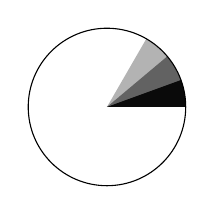
\begin{tikzpicture}
\draw (1,0) arc (0:360:1cm);
\foreach \x in {1,2,3}{
	\onslide<\x>{\fill[opacity=0.9/\x](1,0) arc(0:20*\x:1cm)--(0,0)--cycle;}
	}
\end{tikzpicture}
\end{center}
\StatusBar{1}{3}
\end{frame}
%----------------------------------------------------------------------------------------
%----------------------------------------------------------------------------------------
\begin{frame}{Unobtrusive Notes}
\unote{ $\rightarrow$ Here, in the left-hand corner, by the page number $\leftarrow$}
References to the text are sometimes put next to the page number. 
Content on the slides is similar, but usualy not identical, to the reference. The references can help you track which part of the text corresponds to the current slide.
\vfill

Keen students can investigate the references in the text if they want a longer written explanation, or a similar example to practice on. For that reason, these show up the handouts as well as in beamer mode. 
\end{frame}
%----------------------------------------------------------------------------------------
\begin{frame}
\textcolor{spoilercolor}{Text in this colour in the full or lecture versions of the slides does not show up in the handout version. So, this colour signals that students will only see this text on your screen, and not on their redacted copies.}
\vfill
Sometimes things that look like answers are included in the student handouts. For example, if a question is only included to motivate a theorem, its solution might be included for them, because the question serves more as exposition than as practice. These would be coloured normally.
\end{frame}
%----------------------------------------------------------------------------------------
\begin{frame}
If you just want to use the slides as they are, you can stop here. 
\vfill
The remaining sections describe how to use the custom macros, and are only necessary if you intend to \alert{edit} the slides.
\end{frame}

%----------------------------------------------------------------------------------------
\section{Versioning Macros}
\frame{\tableofcontents[currentsection]}
%----------------------------------------------------------------------------------------
%----------------------------------------------------------------------------------------
\begin{frame}{Versions}
The three versions described in the first section are generated using beamer modes and the spoilers toggle (discussed later).
\begin{center}
\begin{tabular}{|c||c|c|}
\hline
\textbf{version} & \textbf{mode} & \textbf{spoilers}
\\ \hline
lecture & beamer & false
\\ \hline
handout & handout & false
\\ \hline
full & beamer & true
\\ \hline
\end{tabular}
\end{center}
\vfill
The usual overlay specifications for modes, e.g. \texttt{\textbackslash onslide$<$1-3|handout:0$>$\{content\}}, will suffice to differentiate between handout and the other two versions.
\end{frame}
%----------------------------------------------------------------------------------------
\begin{frame}[fragile]{Spoilers}
You can set the toggle `spoilers' to true or false in the preamble. This controls content that might be an unwanted hint for students thinking about an example on their own. Full solutions also tagged as spoilers.\vfill
\begin{verbatim}
\settoggle{spoilers}{true}
\settoggle{spoilers}{false}
\end{verbatim}\vfill

The toggle is automatically set to false for lecture and handout versions, and to true for full versions.\vfill

\end{frame}
%----------------------------------------------------------------------------------------
\begin{frame}{Spoilers in overlays}
There are versions of \texttt{\textbackslash only}, \texttt{\textbackslash onslide}, and \texttt{\textbackslash alert} that have spoiler-specific behaviour.
\begin{description}
\item[\texttt{\textbackslash sonly}] \textcolor{spoilercolor}{(`spoilers-only') works like \texttt{\textbackslash only}, but will only show content if the spoilers tag is true, and colour it}.
\item[\texttt{\textbackslash nsonly}] (`no-spoilers-only') works like \texttt{\textbackslash only}, but will only show content if the spoilers tag is false.
\item[\texttt{\textbackslash sonslide}]  \textcolor{spoilercolor}{(`spoilers-onslide') works like \texttt{\textbackslash onslide}, but will only show content if the spoilers tag is true, andcolour it}.
\item[\texttt{\textbackslash nsonslide}] (`no-spoilers-onslide') works like \texttt{\textbackslash onslide}, but will only show content if the spoilers tag is false.
\item[\texttt{\textbackslash salert}] \salert{(`spoilers-alert') works like \texttt{\textbackslash alert}, but will only show content if the spoilers tag is true.}
\end{description}

\end{frame}
%----------------------------------------------------------------------------------------
\begin{frame}{More complicated overlays}
The macros on the previous slide can be used with overlay specifications as usual: for example, you may write \texttt{\textbackslash sonly$<$1-3$>$\{content\}}. 
\vfill
To differentiate between all three versions, there are macros that take the overlay specifications as mandatory arguments. You may \textit{not} use the usual overlay syntax (with angle brackets) with these.
\begin{description}
\item[\texttt{\textbackslash snshonly\{$a$\}\{$b$\}\{$c$\}\{content\}}] (`spoiler/no spoiler/handout only') will print `content' on slide(s) $a$ in full version, on slide(s) $b$ in lecture version, and on slide(s) $c$ in handout version. (To suppress it from one version entirely, ask it to print on slide 0.)
\item[\texttt{\textbackslash snshonslide\{$a$\}\{$b$\}\{$c$\}\{content\}}] behaves similarly, but as \texttt{onslide} instead of \texttt{only}.
\end{description}
\end{frame}
%----------------------------------------------------------------------------------------
\begin{frame}{Versioning and visual cues}
Visual cues are sensitive to mode and the spoiler toggle. They may be used with overlay specifications, e.g. \texttt{\textbackslash AnswerYes$<$1$>$} or \texttt{\textbackslash QuestionBar$<$1-2$>$\{3\}\{5\}}.
\vfill

The prefixes \texttt{s} and \texttt{ns} will cause them to require spoilers to be true or false, respectively, to be displayed. (See upcoming slides for details.) The modes vary by icon, and were chosen to best fit the context in which they are used. (For example, since handouts don't contain solutions, they never contain `AnswerYes' marks. So, `AnswerYes' is only ever printed in beamer mode, not handout mode.)
\end{frame}
%----------------------------------------------------------------------------------------
\begin{frame}{Versioning and visual cues}

The tables below details all commands that take `s' and `ns' prefixes, and when each results in a visible mark. 
\vfil

\begin{overlayarea}{\textwidth}{5cm}
\only<1>{
\begin{tabular}{|c||c|c|c|}
\hline
\textbf{command} & \textbf{mode} &\textbf{spoiler} & \textbf{versions}\\
\hline \hline 
\texttt{\textbackslash AnswerYes} & beamer & true & full\\ 
\texttt{\textbackslash AnswerNo}&&&\\\hline
\texttt{\textbackslash nsAnswerYes} & beamer & false & lecture\\
\texttt{\textbackslash nsAnswerNo}&&&\\ \hline\hline
\texttt{\textbackslash MoreSpace} &beamer& any &lecture, full \\ 
\texttt{\textbackslash NoSpace} &&&\\\hline
\texttt{\textbackslash sMoreSpace} &beamer& true & full \\
\texttt{\textbackslash sNoSpace}&&& \\\hline
\texttt{\textbackslash nsMoreSpace} &beamer& false &lecture \\ 
\texttt{\textbackslash nsNoSpace}&&&\\\hline
\end{tabular}
}
%
\only<2>{
\begin{tabular}{|c||c|c|c|}
\hline
\textbf{command} & \textbf{mode} &\textbf{spoiler} & \textbf{versions}\\
\hline \hline 
\texttt{\textbackslash StatusBar} & beamer & any & lecture, full \\ \hline
\texttt{\textbackslash sStatusBar} & beamer & true & full \\ \hline
\texttt{\textbackslash nsStatusBar} & beamer & false & lecture \\ \hline\hline
\texttt{\textbackslash QuestionBar} & any & any & lecture, full, handout \\ \hline
\texttt{\textbackslash sQuestionBar} & any & true &  full \\ \hline
\texttt{\textbackslash nsQuestionBar} & any & false & lecture, handout \\ \hline\hline
\texttt{\textbackslash AnswerBar} & beamer & true & full \\ \hline
\texttt{\textbackslash nsAnswerBar} & beamer & false & lecture \\ \hline
\end{tabular}
}
\end{overlayarea}
\end{frame}
%----------------------------------------------------------------------------------------
%\begin{frame}
%You can use \texttt{\textbackslash answer\{$<$A$>$\}} as a shortcut for \texttt{\textbackslash iftoggle\{printsolutions\}\{$<$A$>$\}\{\}}. That macro does nothing else.\vfill
%
%
%The printsolutions toggle also affects the commands: \texttt{\textbackslash SetQuestion\{\}}, \texttt{\textbackslash SetAnswer\{\},\texttt{\textbackslash QuestionBar\{\}\{\}}, \texttt{\textbackslash AnswerBar\{\}\{\}}.
% \textbackslash AnswerYes,  \textbackslash AnswerNo}, and \texttt{\textbackslash AnswerSpace}. \vfill
%
%\end{frame}
%----------------------------------------------------------------------------------------
%----------------------------------------------------------------------------------------
\section{Q\&A macros}
\frame{\tableofcontents[currentsection]}

%----------------------------------------------------------------------------------------

%----------------------------------------------------------------------------------------
\begin{frame}{Sets of Questions}
Sometimes there are sets of questions on a particular topic. You can put these inside a \texttt{QuestionSet} environment,  then give questions inside \texttt{\textbackslash SetQuestion\{\}} and  answers inside \texttt{\textbackslash SetAnswer\{\}}. The answers will be shown or hidden according to the printsolutions toggle. Since handout mode sets the printsolutions toggle to false, answers are automatically hidden in handouts.
\vfill

Each question (in both modes) and each answer (in beamer mode) will show up on one overlay. Question and answer staircase status bars will be printed accordingly. If the set has more than about 7 questions, these bars might overrun the page.
\end{frame}
%----------------------------------------------------------------------------------------

%----------------------------------------------------------------------------------------
\begin{frame}{More Flexible Sets of Questions}
The \texttt{QuestionSet} environment takes care of a lot of things for you (like making the items show up on different slides in a handout, and counting how many there are total). The trade-off is that it might be too restrictive. It can only be in one frame environment, for example, and each question will be on a new overlay.
\vfill
A more general way of getting the staircase Q\&A status bar is to use \texttt{\textbackslash QuestionBar\{$<$a$>$\}\{$<$b$>$\}}
and \texttt{ \textbackslash AnswerBar\{$<$a$>$\}\{$<$b$>$\}}. This will put a staircase status bar showing $<$a$>$ of $<$b$>$ total. You'll probably want to wrap these in an \texttt{\textbackslash only} overlay specification to control where they show up. Unlike \texttt{QuestionSet}, the total size of the status bar is fixed, so you don't have to worry about overrunning margins.\vfill

\texttt{\textbackslash QuestionBar\{2\}\{7\}}
\QuestionBar{2}{7}
\end{frame}

%----------------------------------------
%\begin{frame}
%\AnswerYes
% \texttt{\textbackslash AnswerYes} and  \texttt{\textbackslash AnswerNo} place answer boxes in the lower right-hand corner. To have them show up on only certain slides, you should use overlays, such as \texttt{\textbackslash AnswerYes$<$3$>$}. Do not use  \texttt{\textbackslash onslide} (it won't work) or \texttt{\textbackslash only} (the spacing might be wrong on other overlays).\vfill
% 
%
%% The answer boxes can affect the alignment of a slide.   \texttt{\textbackslash AnswerSpace}  avoids jarring text displacement between overlays by making an invisible box of the same size. (It makes \texttt{\textbackslash only} behave more like \texttt{\textbackslash onslide}.)
%\end{frame}

%----------------------------------------------------------------------------------------
\section{General macros}
\frame{\tableofcontents[currentsection]}
\begin{frame}[t,fragile]
Lecturer cues in the corner won't be placed correctly if you have \verb|\centering| on the page, so use \verb|\begin{center} \end{center}| instead, and put the commands outside.
\vfill
The macros in this category are:
\begin{itemize}
\item \verb|\MoreSpace|, \verb|\NoSpace|
\item \verb|\StatusBar|
%\item \texttt{QuestionSet} environment with \verb|\SetQuestion| and \verb|\SetAnswer| 
\item \verb|\QuestionBar, \AnswerBar|
\item \verb|\AnswerYes, \AnswerNo|
\end{itemize}
\vfill
To have them show up on only certain slides, you should use overlays, such as \texttt{\textbackslash AnswerBar$<$3$>$\{2\}\{2\}}. Do \textit{not} use  \texttt{\textbackslash onslide} (it won't work) or \texttt{\textbackslash only} (the spacing might be wrong on other overlays).
\end{frame}
%----------------------------------------------------------------------------------------
%----------------------------------------------------------------------------------------
\begin{frame}[t]{Slide Clicks}
The command \texttt{\textbackslash StatusBar\{$<$a$>$\}\{$<$b$>$\}} will place a small status bar in the lower-right hand corner of the frame, starting at slide number $<$a$>$ and ending at slide number $<$b$>$.\vfill
Sometimes using \texttt{\textbackslash pause} causes errors, so it's best to use explicit overlay commands like \texttt{\textbackslash onslide}.
\StatusBar{1}{1}
\end{frame}
%----------------------------------------------------------------------------------------

\begin{frame}[t]{Map of Contents}
The mindmap tables of contents aren't automatically generated from the sections in a document. Rather, they are saved in the file \texttt{header\_maps.sty}.\vfill

Each chapter has its own map. You can highlight any number of sections in a chapter. Since numbers don't work in TeX as variable names, sections are labeled with letters: 1 is a or A, 2 is b or B, etc. 
\vfill

The command \texttt{\textbackslash mapofcontentsA\{\textbackslash ab,\textbackslash ac}\} will show the map of contents for Chapter 1 (that's the ``A" in the command itself) with sections 1.2 and 1.3 highlighted (that's the list in the argument). \\

The command \texttt{\textbackslash mapofcontentsC\{\}} will show the map of contents for Chapter 3 (that's the ``C" in the command) with no sections highlighted (since the argument is empty).\\

\end{frame}
%----------------------------------------------------------------------------------------

\begin{frame}[fragile]{Referencing the Textbook}
\verb|\eref{text}{<label>}| and \verb|\eref{prob}{<label>}| allow you to reference labelled items in the textbook and problem book, respectively. The folder XR has the aux files from these texts. When the texts are updated, copying the new aux files to that folder will make all the references in the slides update when they are re-compiled.
\vfill
\verb|\eref{text1}{<label>}| will allow you to reference the CLP--1 textbook.
\vfill

\texttt{\textbackslash unote\{$<$content$>$\}} (where `u' stands both for `under' and `unobtrusive') will put $<$content$>$ next to the footline page number. This format is often used to reference the textbook and problem book.
\unote{$<$content$>$}
\end{frame}

%----------------------------------------------------------------------------------------
\begin{frame}[t]{Attribution}

The index is used to cite copyrighted content. The standard format for setting up a citation of an image is:


\texttt{\footnotesize\textbackslash index\{\textbackslash includegraphics[height=3mm]\{$<$file.png$>$\} $<$picture title (link)$>$ by $<$artist (link)$>$ is licensed under $<$license information (link)$>$\}
}

\vfill

The command \texttt{\textbackslash LastPage} prints an index of copyrighted works included in the file so far. If none have been cited with the \texttt{\textbackslash index} command, it will print nothing.\vfill

\texttt{\textbackslash CCBY , \textbackslash  CCBYtwo , \textbackslash CCBYthree \textbackslash  CCBYNCNDfour,} and \texttt{\textbackslash CCBYNCSAtwo} display and link to their respective licenses.
\end{frame}

%%----------------------------------------------------------------------------------------
\CheckFrame{\textbackslash CheckFrame\{$<1>$\}\{$<2>$\} will print $<1>$, then pause and print $<2>$. The content $<2>$ is hidden from the handout. \vfill
To get the same brown text and frame title, without the proscribed overlays, use \textbackslash checkframe\{\}.\vfill
}{
These frames are used extensively when antidifferentiation is first introduced. In class, the author usually works through the first few in detail, then afterwards uses them as an opportunity to remind students how they can (and should) easily check antiderivatives by differentiating. The purpose of the unusual text colour is to make it clear to students what exactly is being skipped.}
%%----------------------------------------------------------------------------------------
\begin{frame}{Colour Scheme}
The following named colours are used in graphics. \vfill
\begin{tikzpicture}
\foreach \x in {1,2}
{
	\draw[white] (\x*1.5,1) node[shape=circle, fill=C\x, minimum size=1cm]{C\x};
	\draw[white] (\x*1.5,3) node[shape=circle, fill=M\x, minimum size=1cm]{M\x};
	\draw[white] (\x*1.5,5) node[shape=circle, fill=W\x, minimum size=1cm]{W\x};}
\foreach \x in {3,4,5}
{
	\draw (\x*1.5,1) node[shape=circle, fill=C\x, minimum size=1cm]{C\x};
	\draw (\x*1.5,3) node[shape=circle, fill=M\x, minimum size=1cm]{M\x};
	\draw (\x*1.5,5) node[shape=circle, fill=W\x, minimum size=1cm]{W\x};}
\draw (0,1)node{cool}; \draw (0,3)node{mixed}; \draw (0,5)node{warm};
\end{tikzpicture}

\end{frame}
%%----------------------------------------------------------------------------------------
\section{Macros for Specific Sections}
\frame{\tableofcontents[currentsection]}
%%----------------------------------------------------------------------------------------
\begin{frame}[fragile]{Choice table for integration by parts}
When performing integration by parts, one must choose a function to be differentiated, and a function to be antidifferentiated. When this technique is first introduced, the two most obvious choices are presented in a table.
\vfill

Suppose one were trying to use integration by parts to evaluate $\ds\int f(x)g(x)\,\dee x$. One option is to differentiate $f$ and antidifferentiate $g$; another option would be to differentiate $g$ and antidifferentiate $f$.
\vfill

The syntax of the macro is:
\vfill

\small
\verb|\IBP{<variable>}{<f>}{<f'>}{<F>}{<g>}{<g'>}{<G>}{<slide>}|
\normalsize
\vfill

All entries are inputted as text (no dollar signs). In the above scenario, the variable is $x$; $f'$ is the derivative of $f$; $F$ is the antiderivative of $f$, etc. The last argument gives the overlay number on which the table will first appear.

\end{frame}
%%----------------------------------------------------------------------------------------
%%----------------------------------------------------------------------------------------
\begin{frame}[fragile]{Choice table for integration by parts}
The macro
\verb|\IBP{x}{f}{f'}{F}{g}{g'}{G}{1}|
 
generates the table below: \vfill

\IBP{x}{f}{f'}{F}{g}{g'}{G}{1}\vfill

The derivatives and antiderivatives are hidden in the handout, and only show up on the second and third slide here, to give instructor and/or students time to compute them on their own, if desired.
\end{frame}
%%----------------------------------------------------------------------------------------
\begin{frame}[fragile]{Right Triangle}
When we use a trigonometric substitution, we often have to convert between trigonometric functions. For example, suppose we use the substitution $x=\sin \theta$, but then our final answer includes $\tan\theta$. A triangle is often helpful for deciding that $\tan\theta = \frac{x}{\sqrt{1-x^2}}$.\vfill

The command \verb|\TrigTri{<angle>}{<adjacent>}{<opposite>}{<hypotenuse>}| will generate a right triangle with one angle labeled $<$angle$>$, the adjacent side to that angle labelled $<$adjacent$>$, etc.

\end{frame}
%%----------------------------------------------------------------------------------------
\begin{frame}[fragile]{Right Triangle}
The command \verb|\TrigTri{\theta}{}{x}{1}| generates the triangle below:
\vfill
\TrigTri{\theta}{}{x}{1}

\end{frame}
%%----------------------------------------------------------------------------------------
\begin{frame}{Visualizing Series}
The \textbackslash\texttt{weights} macro is intended to impress upon students the relationship between sequences and series. It uses the visual metaphor of weights being added to a scale. Before describing its implementation, we'd like to justify its prevalence, because it is both prominent and repetitive in the slides.
\vfill

For many years, the author dealt with students who, nearing the final exam, would confuse \textit{sequences} with \textit{series}. The concepts aren't hard to tell apart, and students wouldn't confuse them when they were \textit{first} introduced. It was only after they'd been using them for a while that the lines seemed to blur. \vfill

\end{frame}
%----------------------------------------------------------------------------------------

%----------------------------------------------------------------------------------------
\begin{frame}{Visualizing Series}
The author's theory of the source of the end-of-course confusion around sequences is that learners are sometimes manipulating expressions without keeping the \textit{meaning} of those expressions top-of-mind. One becomes engrossed in the mechanics of, say, the ratio test, and forgets what exactly is being tested.\vfill

Since implementing the repetitive display of a visual metaphor, the frequency with which the author was asked the difference between a sequence and a series has decreased dramatically (albeit anecdotally). Explanations about manipulations of partial sums have also become easier, using the shared metaphor of weights on a scale.
\end{frame}

%----------------------------------------------------------------------------------------
\begin{frame}[fragile]{Visualizing Series}
The visual metaphor for a series is that the terms of the series are weights (or helium balloons, if they're negative) on a scale. Putting down one weight at a time and noting the reading on the scale generates the sequence of partial sums.
\vfill
The  \verb|\weights| macro should be called inside a tikzpicture environment. It takes three arguments. The first is a list of the sizes of weights; the second is a list of labels for those weights; and the third is a sequence of partial sums. All are entered as lists.

\end{frame}
%----------------------------------------------------------------------------------------
\begin{frame}{Visualizing Series}{First argument of \texttt{\textbackslash weights}: sizes}

The first argument specifies the relative sizes of weights that should be displayed.
\vfill
The inputted sizes are scaled to make the icons (weights / balloons) fit on the scale. So inputting \texttt{1,.5,.25} should give the same result as inputting \texttt{4,2,1}. There is a minimum space between each icon, so if you put too many terms here, the icons will overrun the right margin of the frame. There is also a maximum size cutoff for each icon, so in a series whose terms rapidly decay, \textit{the first several icons may be the same size}.
\vfill
There are two reasons why these sizes are entered separately from their labels. In addition to specifying formatting, it is often desirable to take some poetic license with the sizes for clarity. A series whose terms decay quickly is hard to sketch realistically.

\end{frame}
%----------------------------------------------------------------------------------------
\begin{frame}{Visualizing Series}{Second argument of \texttt{\textbackslash weights}: labels}
The second argument gives labels to be added to the weights. Each label disappears as the weight drops to the scale.
\vfill
These will be interpreted as being in math mode, so enter \texttt{\textbackslash frac12} instead of \texttt{\$\textbackslash frac12\$}.
\vfill
You do not need to have as many labels as there are weights. Indeed, you can leave the second argument entirely blank, if you choose.
\end{frame}
%----------------------------------------------------------------------------------------
\begin{frame}{Visualizing Series}{Third argument of \texttt{\textbackslash weights}: partial sums}
The third argument gives the sequence of partial sums. Partial sums are displayed one-by-one on the scale, and stored on the right-hand side of the frame, to emphasize the ``sequence" part of ``sequence of partial sums."
\vfill
If you leave the third argument blank, the partial sums will be computed using the list of weight sizes (the first argument in the macro), and truncated to 4 decimal places.
\vfill
By default, the first partial sum is $S_1$. \texttt{\textbackslash setpartialstart\{n\}} will make the first partial sum $S_n$. ($n$ must be an integer, not a parameter.) The default starting index will reset at the end of the frame, or you can use \texttt{\textbackslash resetpartialstart} to reset it.
\end{frame}
%----------------------------------------------------------------------------------------
\begin{frame}[fragile]{Visualizing Series: example 1}{Everything specified; realistic weight sizes, but rapid decay}
The next frame shows the result of:
\vfill

\verb|\begin{tikzpicture}|\\
\verb|\weights{4,2,1}{\frac12,\frac14,\frac18}{.5,.75,.875}|\\
\verb|\end{tikzpicture}|
\vfill

If we're trying to represent $\frac12+\frac14+\frac18$, the weight sizes (first argument) might seem to be realistic, because they are proportional to the actual summands.
\vfill

Because the terms of the sum decay rapidly, displaying the sizes as given makes the first icon huge. So, the first icon is constrained by a maximum size, making it the same size as the second icon. So in the actual display, the sizes of the icons don't correspond well to the summands.
\end{frame}
%----------------------------------------------------------------------------------------
\begin{frame}[fragile]{Visualizing Series: example 1}

\begin{tikzpicture}
\weights{4,2,1}{\frac12,\frac14,\frac18}{.5,.75,.875}
\end{tikzpicture}
\end{frame}
%----------------------------------------------------------------------------------------
%----------------------------------------------------------------------------------------
%\begin{frame}[fragile]{Visualizing Series: example 2}{Everything specified, fake weight sizes}
%The next frame shows the result of:
%\vfill
%
%\verb|\begin{tikzpicture}|\\
%\verb|\weights{6,4,3,2,1}|\\
%\verb|{\frac12,\frac14,\frac18,\frac1{16},\frac1{32}}|\\
%\verb|{.5,.75,.875,2.035,2.06625}|\\
%\verb|\end{tikzpicture}|
%\vfill
%
%If we're trying to represent $\frac12+\frac14+\frac18$, the weight sizes (first argument) are not to scale. In contrast to the last example, the icons all have different sizes. This slight deception makes the image feel more realistic.
%\vfill
%
%We didn't specify labels for every weight.
%\end{frame}
%%----------------------------------------------------------------------------------------
%\begin{frame}{Visualizing Series: example 2}
%
%\begin{tikzpicture}
%\weights{6,4,3,2,1}{\frac12,\frac14,\frac18}{.5,.75,.875,2.035,2.06625}
%\end{tikzpicture}
%\end{frame}
%----------------------------------------------------------------------------------------
\begin{frame}[fragile]{Visualizing Series: example 2}{Unspecified partial sums}
The next frame shows the result of:
\vfill
\scriptsize
\verb|\setpartialstart{0}|
\verb|\begin{tikzpicture}|\\
\verb|\weights{1,.9,.81,.729,.6561,.59049,.531441}|\\
\verb|{1,\frac9{10},\frac{9^2}{10^2},\frac{9^3}{10^3},\frac{9^4}{10^4},\frac{9^5}{10^5},\frac{9^6}{10^6}}|\\
\verb|{}|\\
\verb|\end{tikzpicture}|
\normalsize
\vfill
The first partial sum is labeled $S_0$, instead of $S_1$.
\vfill
The weights (first argument) are written accurately, so we can leave the partial sums (third argument) blank. Note the partial sums are all printed with 4 digits.
\vfill
Because the series decays slowly, it's possible to show all weights with different sizes, without any weight overrunning the system's maximum and being scaled down.
\end{frame}

%----------------------------------------------------------------------------------------
\begin{frame}{Visualizing Series: example 2}
\setpartialstart{0}
\begin{tikzpicture}
\weights{1,.9,.81,.729,.6561,.59049,.531441}{1,\frac9{10},\frac{9^2}{10^2},\frac{9^3}{10^3},\frac{9^4}{10^4},\frac{9^5}{10^5},\frac{9^6}{10^6}}{}
\end{tikzpicture}
\end{frame}

%----------------------------------------------------------------------------------------

%----------------------------------------------------------------------------------------
\begin{frame}[fragile]{Visualizing Series: example 3}{Negative terms,  label sizes}
The next frame shows the result of:
\vfill
\small
\verb|\begin{tikzpicture}|\\
\verb|\weights{1,-.9,.81,-.729,.6561,-.59049,.531441}|\\
\verb|{\displaystyle{\left(-\frac9{10}\right)^0},|\\
\verb|\textstyle{\left(-\frac9{10}\right)^1},|\\
\verb|\scriptstyle{\left(-\frac9{10}\right)^2},|\\
\verb|\text{\scriptsize $\left(-\frac9{10}\right)^3$},|\\
\verb|\text{\tiny $\left(-\frac9{10}\right)^4$}}|\\
\verb|{}|\\
\verb|\end{tikzpicture}|
\normalsize
\vfill
The negative terms are shown as helium balloons.
\vfill
Various commands are shown that can change the sizes of the labels.
\end{frame}

%----------------------------------------------------------------------------------------
\begin{frame}{Visualizing Series: example 3}
\begin{tikzpicture}
\weights{1,-.9,.81,-.729,.6561,-.59049,.531441}{
\displaystyle{\left(-\frac9{10}\right)^0},
\textstyle{\left(-\frac9{10}\right)^1},
\scriptstyle{\left(-\frac9{10}\right)^2},
\text{\scriptsize $\left(-\frac9{10}\right)^3$},
\text{\tiny $\left(-\frac9{10}\right)^4$}}{}
\end{tikzpicture}
\end{frame}

%----------------------------------------------------------------------------------------
%----------------------------------------------------------------------------------------
\begin{frame}[fragile]{Visualizing Series: further details}
\begin{itemize}
\item In handout mode, there is no animation. The slide shows the labelled weights hovering above the scale, and displays the sequence of partial sums.
\item To shorten the animation, use overlay commands, e.g. \verb|\begin{frame}<1,10->|.
\item Infinite sums are represented as finite sums, so it's nice to include a verbal reminder that we imagine this process continuing on.
\item When specifying labels,  note the entire entry gets put into math mode, so simply writing \verb|\small| won't make the labels smaller. 
\begin{itemize}
\item The easiest way to change sizes is to use math styles (like \texttt{\textbackslash displaystyle} or \texttt{\textbackslash scriptstyle}). 
\item Alternately, you can put the entry inside a text bracket, then specify the text size, then put it back into math mode. For example, \texttt{\textbackslash text\{\textbackslash tiny \$\textbackslash frac12\$\}}
\end{itemize}
\end{itemize}
\end{frame}
%----------------------------------------------------------------------------------------
\begin{frame}{Hippo Stacks}
The weights-on-a-scale visualization doesn't lend itself nicely to comparing series, so we provide a second visual metaphor: stacks of hippos. The height of each hippo represents the term being added, so the height of the stack of hippos is a sum. 
\vfill

The macro still needs to be called inside a tikzpicture environment. \texttt{\textbackslash HippoStack} takes two arguments. The first is a list of hippo heights; the second is a list of labels. As with weights on a scale, there can be fewer labels than hippos.
\vfill

\texttt{\textbackslash VarHippoStack} works the same way, but it produces hippos that are a different colour and facing a different direction.
\end{frame}
%----------------------------------------------------------------------------------------
\begin{frame}[t,fragile]{Hippo Stacks}
\scriptsize
 \verb|\begin{tikzpicture}\HippoStack{3,2,1}{label 1,label 2}\end{tikzpicture}|
 \normalsize
\vfill
\begin{tikzpicture}\HippoStack{3,2,1}{label 1,label 2}\end{tikzpicture}
\end{frame}
%----------------------------------------------------------------------------------------
\begin{frame}{Hippo Stacks}
Unlike weights on a scale, the sizes given for hippo stacks are interpreted literally, not scaled to fit the page. Their units are centimetres.\vfill

Also unlike weights on a scale, the labels are interpreted as text, not math. So if you want to use math mode, you'll add the dollar signs to each element on the list.
\end{frame}
%----------------------------------------------------------------------------------------
\begin{frame}[t]
An example using \texttt{\textbackslash smash} to allow the hippos\\ to overrun the frame:

\vspace{7cm}
\smash{\begin{tikzpicture}
\HippoStack{3,2,1}{3,2,1}
\begin{scope}[xshift=5cm]
\VarHippoStack{2.5,
1.25,
0.8333333333,
0.625,
0.5,
0.4166666667,
0.3571428571,
0.3125,
0.2777777778,
0.25,
0.2272727273,
0.2083333333,
0.1923076923,
0.1785714286,
0.1666666667,
0.15625,
0.1470588235,
0.1388888889,
0.1315789474,
0.125,
0.119047619,
0.1136363636,
0.1086956522,
0.1041666667,
0.1,
0.0961538462
}{1,\small $\frac12$,\footnotesize $\frac13$,\scriptsize $\frac14$}
\end{scope}
\end{tikzpicture}}
\end{frame}
%----------------------------------------------------------------------------------------
\begin{frame}{Hippo Stacks}
Further details and tricks:
\begin{itemize}
\item To use multiple stacks, you'll have to separate them yourself. You can make two different pictures environments, or use e.g. \texttt{
\textbackslash
 begin\{scope\}[xshift=5cm]
  $\cdots$ 
  \textbackslash end\{scope\}
}.\vfill

%\item I like the effect of divergent series overrunning the top of the page. \texttt{\textbackslash smash} is helpful there.\vfill

\item To place a large number of hippos, one may wish to generate the desired decimals in a spreadsheet, then copy-paste the list to the .tex file.\vfill

\item The hippo sizes in the slides are, more-or-less,  proportional to the series they are meant to represent. We hope this helps students strengthen their intuition.
\end{itemize}
\end{frame}
%----------------------------------------------------------------------------------------
\begin{frame}{Substitution Rule}
When we did simple examples of the substitution rule, we had special colours for the ``inside" function (usually called $u$) and its derivative. The colour for the differential is meant to stand out more, since it is commonly forgotten by new learners.
\vfill
\begin{itemize}
\item For the inside function: \texttt{\textbackslash su\{text\}} gives  \su{text}.
\item For just the letter 'u':  \texttt{\textbackslash su\{\}} gives  \su{}.
\item For the derivative of the inside function: \texttt{\textbackslash sdu\{text\}} gives  \sdu{text}.
\item For just  '\dee u':  \texttt{\textbackslash sdu\{\}} gives  \sdu{}.
\end{itemize}
The colour in the commands is overlay-aware.
\vfill
In later examples, where these functions were not so easily tracked, we didn't use special colours.
\end{frame}
%----------------------------------------------------------------------------------------
\LastPage
%----------------------------------------------------------------------------------------
%----------------------------------------------------------------------------------------
\end{document}
%----------------------------------------------------------------------------------------
